\documentclass{llncs}

\newif\ifnoTBD \noTBDfalse

% Uncomment to remove TBD macros
%\noTBDtrue

\ifx\pdftexversion\undefined
  \usepackage[dvips]{graphicx}
\else
  \usepackage[pdftex]{graphicx}
  \usepackage{epstopdf}
\fi

\ifnoTBD
\def\TBD#1{\typeout{TBD not done: #1}}
\else
\def\TBD#1{\textcolor{blue}{TBD: #1}}
\AtEndDocument{\typeout{ *** ATTENTION: compilation is in DRAFT
    mode. There might still be TBD that appear in the document ***}}
\fi

\usepackage[usenames]{color}
\usepackage{xspace}
\usepackage{listings}
%\usepackage{type1cm}
\usepackage{eso-pic}
\usepackage{subfigure}
%\usepackage{multirow}
\usepackage{url}
\usepackage{latexsym}
%\usepackage{hyperref}
\usepackage{comment}
\usepackage{algorithmic}
\usepackage{algorithm}
\newcommand{\INDSTATE}[1][1]{\STATE\hspace{#1\algorithmicindent}}

%\hypersetup{%
%  pdftitle={},
%  pdfauthor={George Bosilca},
%  pdfkeywords={network scheduling}
%  bookmarksnumbered, pdfstartview={FitH},
%  linkbordercolor={0 0 0},
%  citebordercolor={0 0 0},
%  urlbordercolor={0 0 0},
%  pdfborder={0 0 0},colorlinks={true},
%  linkcolor={0 0 0},
%  urlcolor=none,
%  citecolor=white
%}%

%\setlength{\oddsidemargin}{0in}   % origin is (1",1") from top-left corner
%\setlength{\evensidemargin}{0.0in}
%\setlength{\textwidth}{6.5in}
%\setlength{\textheight}{9in}
%\setlength{\topmargin}{0.0in}
%\setlength{\headheight}{0pt}
%\setlength{\headsep}{0pt}

\newcommand{\ompi}{Open\,MPI\xspace}
\newcommand{\ftla}{FT-LA\xspace}
\newcommand{\scalapack}{ScaLAPACK\xspace}
%\newcommand{\abft}{Algorithmic Based Fault Tolerance\xspace}
\newcommand{\abft}{ABFT\xspace}
\newcommand{\cof}{CoF\xspace}

\usepackage{algorithmic}
\usepackage{algorithm}
\usepackage{color}
%\usepackage{amsthm}
\usepackage{amsfonts} 
\usepackage{amssymb,amsmath} 
\usepackage{graphicx}
\usepackage[strings]{underscore}

\begin{document}

\title{A Checkpoint-on-Failure Protocol for Algorithm-Based Recovery in Standard MPI}
%\title{Enabling Algorithm-Based Recovery in Standard MPI with Checkpoint-on-Fault}
\author{            Wesley Bland \and
                    Peng Du \and
                    Aurelien Bouteiller \and
                    Thomas Herault \and
                    George Bosilca \and
                    Jack J. Dongarra}
\institute{
                    Innovative Computing Laboratory, University of Tennessee\\
					1122 Volunteer Blvd., Knoxville, TN 37996-3450, USA\\
					\email{\{bland, du, bouteill, herault, bosilca, dongarra\}@eecs.utk.edu}}

\maketitle

\begin{abstract}

As recent research has demonstrated, it is becoming a necessity for large scale
applications to have the ability to tolerate process failure during an
execution. As the number of processes increases, checkpoint/restart fault
tolerance approaches requiring large concurrent state checkpointing become untenable and radically new
methods to address fault tolerance are needed. This work addresses these
challenges by proposing a novel approach to a minimalistic fault discovery and
management model.  Such a model allows application to run to
completion despite fail-stop failures. As a proof of concept, in addition to the
proposed fault tolerance model, an implementation in the context of the \ompi
library is provided, evaluated and analyzed.
% as well as providing a corresponding implementation in the context of the
% \ompi project.  allow applications to discover and tolerate failures while
% continuing execution, all while minimizing application involvement. It
% includes modifications to the \ompi runtime as well as MPI library to give the
% user options when deciding how best to implement fault tolerance.

\end{abstract}


%\begin{IEEEkeywords}
%Fault Tolerance, Message Passing Interface, ABFT, On-Demand Checkpointing
%\end{IEEEkeywords}

\section{Introduction}

The insatiable processing power needs of domain science has pushed High
Performance Computing (HPC) systems to feature a significant
performance increase over the years, even outpacing "Moore's law"
expectations. Leading HPC systems, whose architectural history is listed
in the Top500~\footnote{www.top500.org} ranking, illustrate how massive
parallelism has been embraced in the recent years, leading to ever
growing systems featuring an impressive number of computing units;
current number 1, the K-computer has half a million cores, and even with
the advent of GPU accelerators, it requires no less than 73,000
cores for the Tsubame 2.0 system (\#5) to breach the Petaflop
barrier. Indeed, the International Exascale Software Project, a group
created to evaluate the challenges on the path toward Exaflop class
machines, has published a public report outlining that a massive
increase in scale will be necessary, when considering probable advances
in chip technology, memory and interconnect speeds, as well as
limitations in power consumption and thermal envelope~\cite{iesp}.
According to these projections, as soon as 2014, billion way parallel
machines, encompassing not only millions of cores, but also tens of
thousands of nodes, will be necessary to achieve the desired level of
performance. Even considering extremely optimistic advances in hardware
reliability, probabilistic amplification entails that failures will be
unavoidable, becoming common events. Hence, fault tolerance is paramount
to maintain scientific productivity.

Already, for Petaflop scale systems the issue has become pivotal. On
one hand, the capacity type of workload, composed of a large amount of
medium to small scale jobs, which often represent the bulk of the
activity on many HPC systems, has traditionally been left unprotected
from failures, resulting in diminished throughput due to failures. On
the other hand, selected capability applications whose significance is
motivating the construction of supercomputing systems are protected
against failures by ad-hoc, application-specific approaches, at the
cost of straining engineering efforts, translating in high software
development expenditures. Two long lasting issues have hindered
ubiquitous adoption of streamlined fault tolerance techniques: first,
the traditional checkpoint based approaches incur a steep overhead on
failure-free operations; second, the dominant approach for programming
parallel distributed memory systems, the MPI standard~\cite{MPI22} and
its implementations, offer extremely limited support for software
fault tolerance approaches, which effectively limit the spectrum of
options available to applications to periodic checkpointing and
rollback recovery.

Several propositions have emerged from the ongoing MPI-3
forum\footnote{\url{http://meetings.mpi-forum.org/mpi3.0\_ft.php}},
toward improving the expressivity of MPI with regard of fault tolerant
techniques. However, it is yet unclear as to wether these propositions
will prove successful enough to be blessed by the forum as they still
incur synchronization overhead on failure-free scenarios. The current
MPI-2 standard leaves open an optional behavior to qualify as a "high
quality implementation", regarding failures: according to this
specification in the case of an MPI\_ERRORS\_RETURN error handler,
when the MPI library detects a failure it should return control to the
caller. This is at the opposite of the default mass-suicide action
that all notable MPI implementations undergo in case of a failure. In
this paper, we investigate the modifications that are required, inside
the MPI implementation, to enable this behavior strictly within the
scope of the current standard. We then describe how algorithm-based
recovery techniques, illustrated by the most useful QR factorization,
are able to leverage this behavior, to perform an inexpensive recovery
that completely avoids costly periodic checkpointing, and rollback
recovery. Although the proposed technique uses checkpointing to save
the state of the application, it does so only after the system was
affected by a failure, and the recovery operation could be qualified as forward
recovery, since it does not make the application rollback.

The remainder of this paper is organized as follows. The next section
presents typical fault tolerant approaches and related works to discuss
their requirements and limitations. Then, we present in
Section~\ref{sect:ompi} the On-Demand Checkpointing approach, and the
minimal support required from the MPI implementation. 
Section~\ref{sec:ftla} presents the use case: a fault tolerant
version of the QR algorithm, and how it has been modified to fit the
proposed paradigm. Section~\ref{sec:model} presents a performance model to
assess the efficiency of both periodic checkpointing with rollback
recovery and On-Demand Checkpointing, and
Section~\ref{sec:experiments} presents an experimental evaluation of
the implementation.
%Section~\ref{sec:ompi} investigates
%the intricacies of the MPI runtime



\section{Background \& Related Work}
\label{sect:background}

% Discuss some MPI-3 related proposals and issues

%Among the issues
%raised during the readings of the proposals, were the fact that these
%approaches will still incur a significant overhead on failure free
%operations, by requiring periodic \emph{consensus}

\subsection*{Background}

Message passing is the dominant form of communication used in parallel
applications, and MPI is the most popular library used to implement
it. However, as fault tolerance becomes a growing concern for
application developers, users have encountered some challenges with
the current MPI Standard that limit their options of fault tolerance
methods. The primary form of fault tolerance today is to periodically
write a checkpoint to disk.  While this method is effective in
allowing applications to recover from failures by restarting the work
from a previously saved point, it causes serious concerns on the
scalability~\cite{ExaScaleResilience09}. Moreover, such proactive
approach to fault tolerance requires a good idea of how many faults
might hurt the system, with which frequency and on what nodes. Many
works have discussed the optimal checkpointing period in the hope that
as few as possible of these preventive actions are taken by the
application~\cite{Young:1974, Gelenbe:1979, Plank01, Daly:2006,
  PreventiveCheckpointing11}. Unlike these works, the work presented
here focuses on {\it forward recovery}: checkpoint actions are taken
only {\emph after} a failure is detected, make it unnecessary to
hypothesize on an optimal checkpoint interval. The checkpoint interval
is optimal, by definition, as there will be one checkpoint interval by
effective fault.

An alternative approach to rollback recovery is to take advantage of
the properties of the application to design it as naturally fault-tolerant. This
technique is traditionally called \abft \cite{huang1984algorithm}. The
algorithm itself includes modifications, or additional steps, to cope
with the loss of some of its data. It includes a modification of the
algorithm, usually to maintain redundant information in the data
during the life of the application, and a recovery procedure that
works only with the data remaining after the failure is detected, and
reconstructs the missing data using additional computation and
communication. To support such an algorithm, the underlying
programming environment must however provide a way to communicate
after the failure occurs on one of the processes.

The current MPI Standard (MPI-2.2,~\cite{MPI22}) does not provide
significant help to deal with that type of behavior. Section~2.8
states in the first paragraph: ``\emph{MPI does not provide mechanisms
  for dealing with failures in the communication system. [...]
  Whenever possible, such failures will be reflected as errors in the
  relevant communication call. Similarly, MPI itself provides no
  mechanisms for handling processor failures.}'' Failures, be they due
to a broken link or a dead process are considered as resource
errors. Later, in the same section: ``\emph{This document does not
  specify the state of a computation after an erroneous MPI call has
  occurred. The desired behavior is that a relevant error code be
  returned, and the effect of the error be localized to the greatest
  possible extent.}'' So, for the current standard, process or
communication failures are to be handled as errors, and the behavior
of the MPI application after an error has been returned is left
unspecified by the standard. However, the standard does not prevent
implementations to go beyond its requirements, and on the contrary,
encourages high-quality implementations \emph{to return} errors once a
failure is detected.

Unfortunately, most of the implementations of the MPI Standard have
taken the path of considering process failures as unrecoverable
errors, and the processes of the application are most often killed by
the runtime system, when a failure hits any of them. The runtime
system then returns with an error code, signaling the failure of the
run, leaving no other choice to the user but to run a new parallel
execution.

The MPI forum is currently examining options for the future direction
of MPI for MPI-3. One of the workgroups is dedicated to propose a
standard form of MPI-supported fault tolerance. The proposal outlines
a method of run-through stabilization which allows the application to
acknowledge and repair communications, both collectively and between
specific ranks in a point-to-point way~\cite{Hursey11MPI3FT}. The
emphasis of the proposal is a set of "validation" functions which the
application is required to call to repair and re-enable communication within
an MPI communicator containing a failed process. To repair point to
point wildcard receives, the application needs to collectively call the function
MPI\_COMM\_REENABLE\_ANY\_SOURCE. To repair collective communication
within a communicator, the application needs to call the function
MPI\_COMM\_VALIDATE.  These functions give the MPI implementation an
opportunity to acknowledge failures and discover or ensure that other
MPI processes also acknowledge the same failures. It also gives the
MPI library a chance to repair communication channels between
remaining processes, optimizing communication topologies if possible
and necessary.

While this method of fault tolerance is sufficient for \abft, it is
not without its drawbacks. The calls necessary to recover from
collectives incur a non-trivial overhead even during the fault free
case. MPI\_COMM\_VALIDATE requires a distributed consensus algorithm
which is currently best implemented at log
scale~\cite{Hursey11LogConsensus}. While this level of overhead is
better than the current state of the art of periodic checkpointing, it
still presents a significant cost that not all applications want or
need to pay to check the validity of the communicators. Most
importantly, this proposal does not yet include process recovery,
which is left to a future proposal to the MPI forum.

% Discuss issues in general with FT-MPI like approaches, besides the 
% sheer problem of standard adoption

% Explain why it is not believed that ABFT can perform without REPLACE 
% or BLANK, or leave it for next section ?

\subsection*{Related Work}

FT-MPI~\cite{fagg2000ft} is an MPI-1 implementation which added
extensions to the MPI standard to give users options for their
\abft. FT-MPI proposed to change the MPI semantics of some of the
calls, to enable continuing the execution of the parallel application
after a failure hits the system, and to rebuild the communicators, thus
re-enabling communications. This approach has been proven successful,
and some applications have been implemented relying on the features of
FT-MPI. However, these modifications of the standard were not imported
in the official MPI standard, and no other MPI implementation took the
same approach. The lack of large distribution of the FT-MPI
implementation prevented a large base of users from implementing their
solution based on this proposition.

%  One of
% the solutions implemented in FT-MPI was to introduce a new MPI\_Errhandler
% called MPI\_ERRORS\_BLANK. This MPI\_Errhandler replaced the position of the
% failed processes inside a communicator with MPI\_PROC\_NULL. By using this
% semantic, the remaining MPI calls could function normally as communication with
% MPI\_PROC\_NULL always succeeds. When FT-MPI encountered a fault, it destroyed
% all MPI Communicators and required that the application recreate them to account
% for the failed processes. While this was a useful step in allowing the most
% level of flexibility from the application's perspective, it made recovery very
% complex and added a large overhead.

% FT-MPI is another form of fault tolerance that can be successful for some, but in
% applications that require that all processes be running to reach successful
% completion, having a hole in the communicator is not a valid solution. The
% failed processes need to somehow be recovered.

%\TBD{Anything needed from the QR side of things?}

Besides the works that have been cited previously to present the
problem statement, the different approaches that have been proposed,
and how this approach is original, the article by W. Gropp and E. Lusk
in 2004 \cite{Gropp:2004:FTM:1080704.1080714} is the work closest to
the On-Demand Checkpointing, from the MPI requirement perspective.  In
this article, the authors explain how the standard can be interpreted,
or slightly modified, to allow for a form of fault tolerance. They
consider different approaches: periodical checkpointing; using
inter-communicators and separate MPI applications to contain an error
in an MPI application; modifying the MPI semantics; or propose new
extensions. However, the last three propositions demand more from the
MPI implementation than we require in this work: for example, the MPI
library is supposed to continue its normal execution, if the error was
located in another MPI application, connected with the one subject to
the error through an inter-communicator. In our work we do not even
require such a step: the only
demand on the MPI implementation is that it does not forcibly kill the
living processes without letting them take a checkpoint, but returns
an error. Once this is ensured, no requirement from any MPI call is
needed.

Moreover, we illustrate the well soundness of our approach using a
non-trivial algorithm: a QR factorization, that is made fault tolerant
using the modified \ompi, and the On-Demand Checkpointing
technique. We demonstrate that this approach is functional, and
evaluate its performance at large scale.

\section{Enabling Software Fault Tolerance in MPI}
\label{sect:ompi}

% Issues that need to be fixed in ompi to enable just 
% error-return, don't explain how we use it yet, leave it for next 
% section

\subsection{Errors in MPI and On-Demand Checkpointing}

Contrary to all the proposed additions to the MPI standard introduced
in Section~\ref{sect:background}, we advocate in this paper that an
extremely efficient form of fault tolerance can be implemented, based
on the MPI standard, for those applications which can take advantage
of it. According to the paragraphs of the standard cited in the
previous section, when implementing a high-quality MPI library, the
application should regain control following a process failure.  This
control gives the application the opportunity to save
its state and exit gracefully, rather than the usual behavior of being
aborted by the MPI implementation itself. In most current MPI
implementations, MPI\_ERRORS\_ABORT is the default (and often, only
functional) MPI\_Errhandler.  However, the MPI standard also defines
another handler called MPI\_ERRORS\_RETURN. This handler
should perform any necessary cleanup at the library level and then
return to the application, giving it the opportunity to continue if
possible. The MPI standard does not require that any MPI function
calls continue to operate after an error is returned (thus after a
failure), but even without MPI calls, we will show that it is possible
for the application to complete its computation, or save enough
information after the failure is detected to allow for continuing the
computation in a new application.

\abft algorithms are capable of restoring missing data from redundant
information located in the other processes. This requires, of course,
to communicate between processes, and we acknowledge that requiring
from the MPI implementation to maintain functioning MPI calls after a
failure hit one of the nodes is too demanding in front of the current
standard. However, expecting that the living processes continue to
work after a failure, and to be able to access the other functionalities
of the system seems significantly less perturbing for the MPI
implementors. We will present in the second part of this section how
this was done in the \ompi implementation.

\begin{figure}
\begin{center}
\includegraphics[width=.9\linewidth]{figures/idea.pdf}
\caption{Execution diagram of an On-Demand Checkpointing approach with
  one failure\label{fig:idea}}
\end{center}
\end{figure}

Under this assumption, consider the figure~\ref{fig:idea}. Horizontal
lines represent the execution of different processes in two successive
MPI applications. Living processes are allowed to call any other type
of operations that does not depend on MPI after a fatal error is
returned. In the proposed general approach, processes that detect a
failure will stop immediately to use MPI, save, on a file (local or
remote, depending on the machine capability), all necessary
information to proceed with the \abft algorithm and exit without
calling MPI\_Finalize. This operation does not require communication
if a filesystem, or any other way to do Input/Output operations remains
available. Because process exiting will be considered as failed from
the MPI perspective, all processes of the MPI application will
eventually discover the initial failure, and the application that was
hurt by a failure will then terminate. The user (or a controlling
script), that launched the MPI application in the first place, can
detect the failure by checking the return code of the MPI runtime
system.

Usually, the execution is terminated at this point. However, the user
or the script can launch a new MPI application on the same
resources. This new application will load the local states (second
series of lines in the figure), when available. If the file is not
available, it means that it was not saved for the requesting ranks,
and thus that these ranks were the ones hit by a failure in the
previous run. In the new MPI application, the MPI system is
functional. So, communications are enabled, and the recovery procedure
of the \abft approach can be called to restore the data of the
process(es) that did not find it locally. From this point on, the
application can continue its normal execution, as the global state has
been restored by the \abft recovery procedure. If another failure hits
the system again during the recovery, the local states are not
updated, and the relaunch starts from the beginning. If another
failure hits the system after the \abft recovery, the same procedure
is followed to handle it.

\subsection{On-Demand Checkpointing and Rollback Recovery}

An On-Demand Checkpointing application behaves similarly to the
familiar checkpoint/restart approach. However, by not periodically
saving a checkpoint to stable storage, the application gains an
enormous overhead reduction. Rather than needing to tune an optimal
checkpoint interval and periodically save that checkpoint to stable
storage, the application only needs to save the ``checkpoint'' once
after the failure has already occurred. This has the added benefit of
incurring zero checkpoint-related overhead in the fault-free case, a
consideration that is very important on reliable systems with a low
likelihood of failure.  This means that the same code can be run on
both reliable and non-reliable hardware without modification. This
method of on-demand checkpointing gives the user a safe place to write
its checkpoint before being aborted by the MPI library.

In traditional checkpointing, a complete set of checkpoints is saved
periodically. With on-demand checkpointing, the failed processes will
not write their checkpoints as they have already failed and will most
likely be unable to do so (although link failures could be taken into
consideration: in this case, all processes are able to save the local
state, and the recovery procedure will simply consist in determining
the global state at the moment of failure). Because of this, the
algorithm will need to be able to recover the failed process and
generate all necessary information to bring it back up to the same
point as the other non-failed processes.

There is another fundamental difference between On-Demand
Checkpointing and Coordinated Checkpointing, or most of the rollback
recovery approaches. In traditional rollback recovery, the checkpoint
images must be saved to a reliable media. It is, in particular,
critical to recover the checkpoint image of the failed process to
ensure the recovery. In \cite{HierarchicalCheckpoint09} it is proposed
to keep a local copy of the checkpoint image for the living processes,
if local storage is available, in order to reduce the I/O stress on
the remote storage system, but the failed process must have their
images stored remotely. Since the system does not know what processes
are going to fail at the time of checkpoint, all images must be also
stored remotely. Thus, the (distributed) checkpoint can be considered
complete only when all processes have stored their image on a resource
that has a low probability to fail simultaneously with them. 

In the case of On-Demand Checkpointing, the situation is completely
different: only the checkpoint image of the living processes at the
moment of failure is required. Thus, local storage can be considered
if the same resources can be reused for the restarted MPI
application. Similarly, traditional rollback recovery cannot rely on
local caching of the shared filesystem, while On-Demand Checkpointing
can use this operating system feature to accelerate significantly the
time it takes to save the checkpoint image, and reload it, if memory
is available.

The cost of the On-Demand Checkpointing approach is of course similar
to the cost of any \abft approach: the application might need to do
extra computation during the whole execution, to maintain internal
redundancy that will enable it to restore the missing data when a
failure hits any of the nodes. However, \abft techniques often have an
excellent scalability. For example, the \abft QR operation that we use
to illustrate On-Demand Checkpointing in this work has an overhead on
the fault-free execution inverse proportional to the number of
participating processes, and therefore nodes.
% that decreases when the number of nodes increases.

% Implementation details, might go to a separate section before 
% experiments though, we have room, that would better separate concept 
% from details. 

\subsection{\ompi Implementation\label{sec:mpi}}

\ompi is an MPI 2.2 implementation architected such that it contains
two main levels, the runtime (ORTE) and the MPI implementation (OMPI),
with an additional level to provide support to the other two
(OPAL). As with most MPI library implementations, the default behavior
of \ompi is to abort after a process failure. This policy was
implemented in the runtime system, preventing any kind of decision
from the MPI layer, or the user-level. The major change implemented
for this work was to make the runtime system resilient, and leave the
policy decision in case of failure to the MPI library, and ultimately
to the user application. To do so, we included an incarnation number
in the process names, as they are known by the runtime
system. Incarnation numbers are used to count how many times a process
has failed and are necessary to track the status of all of the
processes in order to know which processes are alive, which have
failed, and reconcile contradictory views. Once the incarnation numbers
are included in the runtime layer, the runtime error manager needs to
change its default behavior during a failure. Rather than notifying
the head node process (HNP) and starting an abort, we introduced a
notification phase, where all runtime processes are notified of the
failure so they can propagate this information to the MPI layer which
appropriately handles the failure according to the application's
instructions.

The runtime layer provides an out-of-band communication mechanism
(OOB) that relays messages through a routing policy implemented in the
routed component. This OOB layer is used to detect failures at the
runtime level, and propagate the failures notifications. We have
changed the routing algorithms to allow for a more dynamic network,
were processes of the OOB can leave the network due to a failure. The
underlying routing algorithm also has a significant influence on the
time it takes to detect a failure and notify all MPI processes, as the
experiments will show.

Like the runtime layer, the OMPI layer has a default behavior during a
process failure of calling MPI\_Abort. The alternative error handler
MPI\_ERRORS\_RETURN is made functional by receiving the failure
notification from the runtime system. When the case happens, all
outstanding communication requests involving the communicator with the
failed process are cancelled. This prevents any outstanding
communications with the failed process from causing a dependency issue
with future communications and ensures that the application will be
notified of the process failure when the MPI function that it is
calling returns a non-MPI\_SUCCESS error code.

In addition to allowing the application to select the MPI\_Errhandler
MPI\_ERRORS\_RETURN, the application can choose to implement custom
MPI\_Errhandlers, another feature of the current MPI standard. In
these custom MPI\_Errhandlers, the application can immediately perform
any post-failure operations, such as saving the local state. These
custom MPI\_Errhandlers provide enormous flexibility to the user.

\section{Example: the QR Factorization}
\label{sec:ftla}

In this section, we propose to illustrate the applicability of \cof by
considering a representative routine of a widely used
class of algorithms: dense linear factorizations. The QR factorization
is a cornerstone building block in many applications, including solving
$Ax=b$ when matrices are ill-conditioned, computing eigenvalues, least
square problems, or solving sparse systems through the GMRES iterative
method. For an $M\times N$ matrix $A$, the QR factorization produces $Q$ and
$R$, such that $A=QR$ and $Q$ is an $M\times M$ orthogonal matrix and
$R$ is an $M\times N$ upper triangular matrix. The most commonly used
implementation of the QR algorithm on a distributed memory machine comes
from the ScaLAPACK linear algebra library~\cite{dongarra1997scalapack},
based on the block QR algorithm. It uses a 2D block-cyclic distribution
for load balance, and is rich in level 3 BLAS operations, thereby
achieving high performance.

%$Q$ is stored
%under the lower diagonal of the input matrix in the form of a $WY$
%representation of the Householder transformation
%products~\cite{schreiber1989storage,bischof1985wy}.

\subsection{\abft QR Factorization}

In the context of FT-MPI, the ScaLAPACK QR algorithm has been rendered fault
tolerant through an \abft method in previous work~\cite{pengduppopp12}. This
\abft algorithm protects both the left ($Q$) and right ($R$) factors from fail-stop
failures at any time during the execution.  At the time of failure, every surviving process is notified by FT-MPI. FT-MPI
then spawns a replacement process that takes the same grid coordinates in the
$P\times Q$ block-cyclic distribution. Missing checksums are recovered from
duplicates, a reduction collective communication recovers missing data blocks in
the right factor from checksums. The left factor is protected by the Q-parallel
panel checksum, it is either directly recovered from checksum, or by
recomputing the panels in the current Q-wide section
(see~\cite{pengduppopp12}). Although this algorithm is fault tolerant, it
requires continued service from the MPI library after failures -- which is a
stringent requirement that can be waived with \cof.

\subsection{Checkpoint-on-Failure QR}

\paragraph*{Checkpoint Procedure:} In our current implementation of
\cof, system-level checkpointing is not supported and would result in
restoring the state of the broken MPI library upon restart. Instead, the
application provides a custom MPI error handler, which invokes an
algorithm specific checkpoint procedure to dump the matrices and the
value of important loop indices into a file.

\paragraph*{State Restoration:} In the theoretical version of the \abft
algorithm, regardless of when the failure is detected, the current
iteration is completed before entering the recovery procedure, so that
all updates are applied to the checksums. In the case of the \cof
protocol, failures interrupt the algorithm immediately, the current
iteration cannot be completed due to lack of communication capabilities.
A ScaLAPACK program has a deep call stack, layering functions from
multiple software packages, such as PBLAS, BLACS, LAPACK and BLAS.
Because failure notification happens only in MPI, lower level, local
procedures (BLAS, LAPACK) are never interrupted. However, PBLAS
operations may be incomplete, and therefore checksums only partially
updated.

To resolve this issue, the call stack must be restored on every process.
The current indices in the loop nest of the QR algorithm, down to the
PBLAS level, are adjunct to the checkpoint. When restarted from a
checkpoint, a process undergoes a ``dry run'' phase that mimics the
already completed loop nests, without actually applying modifications to
or exchanging data. When the same loop indices as before the failure are
reached, the matrix content is loaded from the checkpoint; the state is
then identical to that immediately preceding the failure. The regular
\abft recovery procedure can then be applied: the current iteration of
the factorization is completed to update all checksums and the dataset
is finally rebuilt using the \abft reduction.

\begin{comment}
	
A special situation where failure occurs during 
lower level routines such as PDLARFB is also addressed. This critical 
situation has not been  
covered by any previous work for the complexity it introduces.
	
\subsection{Failure in PBLAS routines}
An important condition for the effectiveness of \abft is the
completion of the current iteration. When a failure interrupts the
program execution during an iteration, the checksum ends up in
intermediate form and as a result cannot be used for recovery.  This
problem worsens when a failure occurs during a lower level routine, 
like a PBLAS, causing a partial trailing matrix update. In this case, updates have been applied to parts of the dataset, possibly without having updated accordingly the corresponding checksums. In the case of the QR algorithm, this problem
is solved by saving the local state when a failure is detected in
PDLARFB rather than in PDGEQRF. The recovery
process in this case is described as follow.

\begin{figure}[b]
	\centering
	\subfigure[After the first step: $A_{2}^{T}V$]{\label{fig:gull1}\includegraphics[totalheight=0.15\textheight, width=0.18\textwidth,viewport=10 10 360 360, clip]{figures/pdlarfb_step1}
	\label{fig:pdlarfb_step1}}
	%\line(0,1){100}
	\subfigure[$A_{2}-V\tilde{W}^{T}$]{\label{fig:gull2}\includegraphics[totalheight=0.15\textheight, width=0.3\textwidth,viewport=10 10 600 360, clip]{figures/pdlarfb_step2}
	\label{fig:pdlarfb_step2}}
	\caption{PDLARFB}
\end{figure}

As shown in Equation (\ref{eqn:qr-trailing}), the trailing update of QR carries
out operation $Q^{T}A_{2}=(I-VT^{T}V^{T})A_{2}\rightarrow
\tilde{A}_{2}$. The right arrow means the updated trailing matrix is
written in-place to $A_{2}$. The trailing matrix update of QR is
similar to PDGEMM for LU which has been shown to hold the checksum
relationship only at the end~\cite{pengduppopp12}. Therefore the procedure
to recover from a failure in PDLARFB is:
\begin{enumerate}
\item Survived processes mark the progress and dump critical data to disk 
\item After re-spawning, all processes dry-run to the failure point
\item All except the replacement process load checkpoint from disk 
\item All processes resume computing from the failure point to the end of PDLARFB
\item At the exit of PDLARFB, recover all lost data in checksum and the whole matrix
\item Execution of PDGEQRF returns to normal
\end{enumerate}
The 'dry-run' step is to re-establish the calling stack of all processes to
the failing point. Therefore PBLAS and ScaLAPACK routines for
computing, for example, PDGEQR2, PDLARFT, etc. are skipped over during 
the dry run.

The recovery is demonstrated with an example of a $4\times 4$ blocks
matrix on a $2\times 3$ grid where failure occurs during PDLARFB.

PDLARFB implements $Q^{T}A_{2}=(I-VT^{T}V^{T})A_{2}$ in three steps:
\begin{enumerate}
\item $W\leftarrow V^{T}A_{2}$
\item $\tilde{W}\leftarrow W\times T$
\item $\tilde{A}_{2}\leftarrow A_{2}-V\tilde{W}^{T}$
\end{enumerate}
Suppose the failure occurs right after step 1 on process (1,0). 
In step 1, as shown in figure~\ref{fig:pdlarfb_step1}, $V$ is stored
in the green trapezoid and $A_{2}$ is in the yellow blocks. $V$ is
first broadcast row-wise to all columns, then GEMM is called on each
process that owns $A_{2}$ with the local $V$ and $A_{2}$. Finally, the
result is produced with column-wise block summation and the result is
stored on the first row of processes that process the first row of
$A_{2}$ (blue blocks).  From the MPI facilities presented in
Section~\ref{sec:mpi}, the failure location is broadcasted to all 
surviving processes and matrix data are dumped to the disk, including
peripheral data like the TAU array and workspace. Surviving processes
also keep a record on whether they have finished the DGEMM in step 1.

After critical data is saved to disk, the program exits and is
re-spawn with a replacement process in the failed process's
location. The re-launched program dry-runs to the failure point in
step 1 of PDLARFB. All previously surviving processes load their
checkpoint from disk while the replacement process stays with its
blank data. Then the program resumes execution of PDLARFB. Since
failure is on process (1,0), $W$ survives the data loss.

Step 2 of PDLARFB is $W\times T$ where $W$ is the blue blocks in
figure~\ref{fig:pdlarfb_step1} and $T$ is a $nb\times nb$ upper
triangular matrix.  Since $T$ resides on each process in the row that
owns $W$, the correctness of $T$ can be always guaranteed, and
therefore $\tilde{W}$ has no lost block in it after calling
DTRMM. $\tilde{W}$ is broadcasted column-wise for step 3.

Step 3 of PDLARFB is shown in figure~\ref{fig:pdlarfb_step2}. In
$\tilde{A}_{2}\leftarrow A_{2}-V\tilde{W}^{T}$, besides
$\tilde{W}^{T}$, $V$ is also correct since $V$ has been broadcast
row-wise to all process in step 1, therefore even if blocks of $V$ are
destroyed by the failure, the result on the replacement process can be
recovered from its neighbor processes in the same row. The result of
step 3, also that of PDLARFB, is affected by the incorrect result in
$A_{2}$, expressed in shadowed blocks in
figure~\ref{fig:pdlarfb_step2}. These incorrect blocks remain in the
result of DGEMM in this step. They are fixed later in the recovery process
in PDGEQRF using both the ABFT and Q-parallel checksum.

For PDLARFB, both $V$ and $T$ can be guaranteed correct no matter when
and where failure occurs, the only variable factor is $W$. However if
the failure does punch holes in $W$, more shadow blocks appear in
the result of PDLARFB, and they can still be fixed by the recovery in
PDGEQRF.
\end{comment}

\section{Models of Fault Tolerance Approaches\label{sec:model}}

In this section, we present a simple model that can be used evaluate the
efficiency of our approach and its behavior under specific circumstances
that are not accessible yet to direct experimentation. For the
following, we will consider an application with a fixed number of
processes, and a fixed amount of work to execute. We consider that
without any fault-tolerance approach enabled, the execution time of this
work with this number of processes is $T$.
%
The execution time of an application managed with the \cof approach 
can be characterized with a few parameters:
\begin{itemize}
\item $C$, the time it takes the living processes, to save their state after the
  failure occurs, exit, and for the runtime system to discover that all
  processes have exited with an error code
\item $\alpha$, a multiplicative factor, that encompasses all costs related to
  making the operation ABFT-capable. Such modification of the operation
  introduces additional operations and communications, distributed among the
  processes. Based on our experience with ABFT, we consider, in this model, that
  these operations introduce a slowdown of the execution time that can be
  captured with a single multiplicative factor, $\alpha > 1$, 
  representing the slowdown on the execution time. As this is inherently 
  tied to the type of fault tolerant approach used in the application, 
  other algorithms may behave differently and require a different modeling 
  of the slowdown. 
\item $R$, the time it takes for processes to restart from scratch, load the
  state of all the processes alive at the last failure, and recover the missing
  data (the data lost due to the failure of a process)
\end{itemize}
Since the number of processors and the problem size are fixed, $C, R,$
and $\alpha$, can all be considered as constants. The downtime incurred 
by provisioning a replacement resource is ignored from the model for two
reasons. First, it can be reduced to a negligible overhead (same order 
of magnitude as the failure detection time, presented in 
Section~\ref{sec:experiments:fd}), simply by reserving some nodes of the 
machine as spares immediately available to replace a failure on any 
application currently running. Second, it can be integrated into $R$ 
without loss of generality, in cases it cannot be neglected. 


Our approach is deterministic, given these assumptions: the time it takes to
complete the execution of the work with a number $n$ of failures is
\begin{eqnarray}
T^{CoF}(n) &=& \alpha T + n ( C + R )
\end{eqnarray}

Indeed, the execution is slowed down by the $\alpha$ parameter to
maintain the different checksums incurred by the ABFT approach, and
each failure triggers first a \cof checkpoint phase, that is immediately
followed by a recovery phase. At the end of the recovery phase, the
algorithm is ready to proceed at the step that follows the failure, so
no additional cost is incurred.

\begin{comment}
The periodical coordinated blocking checkpointing technique can be characterized
with the following parameters:
\begin{itemize}
\item $c$, the time it takes for all processes to save their state
  when the timer expires
\item $r$, the time it takes all processes to restart from this
  checkpoint (load the checkpoint from file)
\item $t$ is the time interval between two checkpoints. This value is
  usually set to something as close as possible to the expected MTBF,
  to avoid unnecessary overheads. It must be set low enough, though,
  to allow for progress.
\end{itemize}
In the coordinated checkpointing approach, the duration of the
execution depends upon the moment of the failures: if a failure hits
the system just after a checkpoint, little time is spent recomputing the
lost progress between the last checkpoint and the failure step. If a
failure hits the system just before a checkpoint,
then the recovery restarts from the last checkpoint and the last
time interval must be entirely re-executed. To model this, we define
two extreme cases: the best case, noted $T^{CC}_B(n)$ (for Time,
Coordinated Checkpointing, Best case), and $T^{CC}_W(n)$ (for Time,
Coordinated Checkpointing, Worst case). These functions can be defined
recursively as follows:
$$
\left\{\begin{array}{l}
T^{CC}_B(0) = T + c T/t\\
T^{CC}_B(n) = T^{CC}_B(n-1) + r + c r/t\\
\end{array}\right.$$
$$\left\{\begin{array}{l}
T^{CC}_W(0) = T + c T/t\\
T^{CC}_W(n) = T^{CC}_W(n-1) + r + t+ c (r+t)/t\\
\end{array}\right.
$$

The cost on the execution without failures is to stop the execution
every $t$ times units, and take a checkpoint. The recovery cost
depends upon the case that is considered. In the best case, all
failures will happen just after the last valid checkpoint. Hence the
cost of recovery will be simply the time to load this checkpoint. In
the worst case, all failures will happen just before the next
checkpoint is completed, hence the cost of recovery will be the time
to load the checkpoint, plus the time to redo the missing part of the
execution, every time. Since recoveries increase the duration of the
execution, they also increase the total number of checkpoints that are
taken.

We can solve these recursive definitions to obtain the following
general forms:
\begin{eqnarray}
T^{CC}_B(n) &= & (c+t)(n r +T)/t\\
T^{CC}_W(n) & = & (c+t) (n (r+t) + T) /t
\end{eqnarray}

To compare the two models, we can assume that if a local storage is
present, $C \ll c$: in the case of the ABFT approach, if the same nodes
remain accessible to the application to restart its runs, and a local
storage is accessible, saving the checkpoint will be a local,
embarrassingly parallel, operation. The Coordinated Checkpointing
approach, however, cannot rely on local storage: a checkpoint image of
all the nodes, including the failed nodes, will be necessary at recovery
time. Thus, in the best case, with local storage, a "buddy algorithm",
where each node stores the checkpoint of a neighbor node; therefore,
supplementary communications are added to the checkpointing time which
is expected to be larger in that case.

On the other hand, if a local storage is not accessible, one can safely
assume that $C \sim c$, since they save the same amount of information
(we are considering a user-level checkpointing in both cases). The \cof
protocol spares the cost of saving the checkpoint of the failed
processes, which could decrease the pressure on the I/O subsystem;
however, as the number of simultaneous failures is assumed very small
compared to the total number or processors, this effect is neglected
here.

% We cannot account for Incremental checkpoint in CC (depends on t, makes c
% (potentially) smaller than C)

Similarly, if no local storage is available, $R \gg r$: they both
incur the communication cost linked to loading the checkpoint image,
but then the ABFT technique needs to introduce additional
communications to recover the state. If a local storage is available,
this will strongly depend on the amount of data saved, and the amount
of communication required by the ABFT algorithm to implement its
recovery. 

Both models present a linear progression with the number of
faults. When $n=0$, the On-Demand Checkpointing approach slowdown
is the factor $\alpha$, while the slowdown in the periodical Checkpointing 
approach is proportional to $(c+t)/t = 1+c/t$. As was
demonstrated in~\cite{lawn253}, $alpha$ decreases when the number of
processes increase. In the case of the QR factorization, it increases
with the square root of the problem size, to maintain the checksum
operation. $c/t$ is proportional to the duration of the checkpoint
operation, hence to the problem size, and in non-scalable storage
system with the number of processes. Moreover, it is highly dependent
on the $t$ parameter, that is often set conservatively to guarantee
progress in case of failures.
\end{comment}

When the system is subject to failures, the cost of the recovery of the
On-Demand Checkpointing technique is proportional to the number of failures, and
to the duration of the recovery, $R$. As stated above, this overhead depends on
the disk capabilities, but also on the efficiency of the recovery procedure
given by the \abft algorithm, and on the runtime system of the MPI to detect the
incomplete termination, and launch a new application, efficiently. In the case
of $QR$, this recovery increases with the size of the problem and the square
root of the number of computing elements. The periodical checkpointing approach
on the other hand incurs a recovery cost that is constant, but must redo part of
the execution. A large $t$ parameter in this case is damageable because it
increase the probability that a long part of the computing time is lost. The
On-Demand Checkpointing technique does not suffer from this parameter, and the
cost of recovery is entirely defined by the size of the problem and the number
of processors.

\section{Performance Discussion} \label{sect:experimental}

\begin{figure*}[t]
  \centering
  \subfigure[\small One Process failing at a time]{
    \label{fig:onebyone}
    \includegraphics[scale=0.65]{figures/even.pdf}
  }
  \subfigure[\small Two concurrently failing processes]{
    \label{fig:burst}
    \includegraphics[scale=0.65]{figures/burst.pdf}
  }
  \caption{Token Roundtrip Time with Evenly Failing Processes}
  \label{fig:even}
\end{figure*}

%\begin{figure*}[t]
%  \centering
%  \subfigure[\small N/2 Processes Failing at Midpoint]{
%    \label{fig:major}
%    \includegraphics[scale=0.50]{major.pdf}
%  }
%  \subfigure[\small N-2 Processes Failing at Midpoint]{
%    \label{fig:critical}
%    \includegraphics[scale=0.50]{critical.pdf}
%  }
%  \caption{Token Roundtrip Time with Many Simultaneous Failing Processes}
%  \label{fig:many}
%\end{figure*}

\begin{figure*}[t]
  \centering
  \subfigure[\small Detection Time for Failures]{
    \label{fig:detection}
    \includegraphics[scale=0.65]{figures/epochs-lines.pdf}
  }
  \subfigure[\small Overhead Introduced by Changes]{
    \label{fig:overhead}
    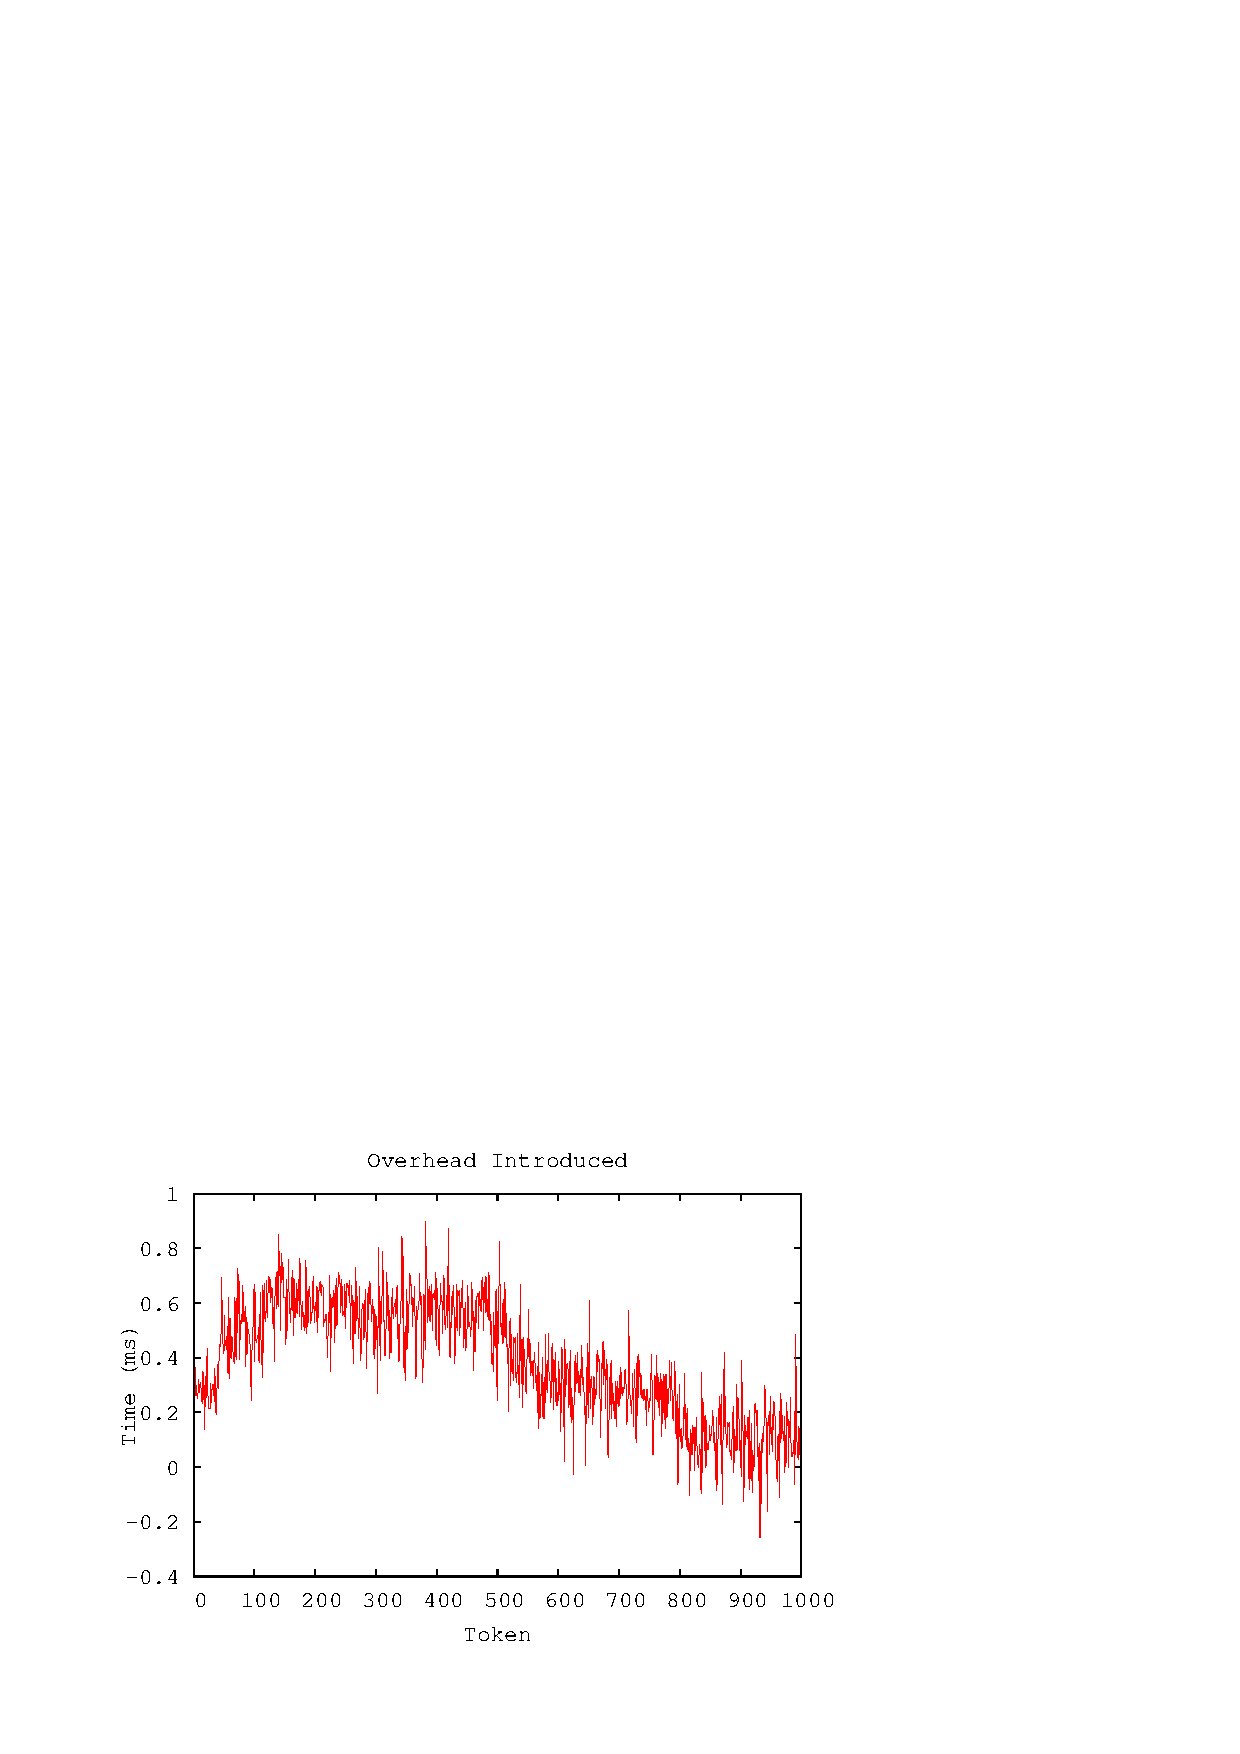
\includegraphics[scale=0.65]{figures/overhead.pdf}
  }
  \caption{Overheads of the Resilient Runtime}
  \label{fig:overheads}
\end{figure*}

% -- Runtime --
In this section we describe the results of our work to this point. First we present a model
to describe the expected results of our resilient runtime's failure notification
method. Second, we will demonstrate the observed values derived from our tests
performed on a 64 node cluster within Grid5000. \footnote{Experiments presented
in this paper were carried out using the Grid'5000 experimental testbed, being
developed under the INRIA ALADDIN development action with support from CNRS,
RENATER and several Universities as well as other funding bodies (see
https://www.grid5000.fr)}

\subsection{Performance Model} \label{subsect:performance_model}
% Describe the model that our runtime is expected to fit within.

We devised a model of the expected failure detection behavior of our runtime
system. Let $T$ be the initial routing topology of the system. Let $L_T(d, f,
H)$ be the time it takes process $d$ to notice a failure of process $f$, knowing
that $\forall q\in H$, $q$ is also failed (potentially before $f$). We call
$L_T(d, f, H)$ the latency of detection of $d$ for $f$ knowing $H$.

$$L_T(d, f, H) \leq \alpha_0 + \gamma D_{T \backslash H \cup \{f\}}(f, d)$$

Where $\alpha_0$ is the time taken by an immediate neighbor of $f$ to detect its
failure, $\gamma$ is the point-to-point message latency, and $D_{T \backslash H
\cup \{f\}}(f, d)$ is the distance (in number of hops) between $f$ and $d$ in
the routing topology, $T \backslash H\bigcup \{f\}$. Note that this distance
could shrink as processes between $f$ and $d$ in the routing topology fail.

Whatever the history of failures $H$, if $|T| = n$, then $D_{T \backslash H}(s,
d) \leq \log_2(n)$. This is true because the routing layer we use is a binomial
tree, which has a maximum depth of $log_2(n)$. Also, when repairing the routing
tree after a failure, the routing layer does not add new hops, it only mends the
routes by removing failed processes from the topology and creating links between
the next surviving neighbors both above and below $f$. Thus, for system $Bin(n)$
with $n$ processes initially, with a fault tolerant binomial tree routing layer,

$$\forall d, f\in Bin(n), \forall H \subseteq Bin(n),$$
$$L_{Bin(n)}(d, f, H) \leq \alpha_0 + \gamma \log_2(n)$$

This shows that our improved routing topology should perform no worse than a
fault free one following a process failure.

\subsection{Performance Data} \label{subsect:performance_data}

% Ring test with binomial routing
% Emphasize "Proof of Concept" rather than large scale performance runs

When validating the runtime work described in Section~\ref{sect:runtime}, our
goal was to devise a test that would confirm its correctness while being simple
to describe and understand. It should be emphasized that this is not necessarily
representative of a specific application, but it does demonstrate that the
improved runtime would be able to support a full application in the presence of
a process failure. It is designed to show that the runtime can heal its routing
layers following multiple and catastrophic process failures. Once a resilient
MPI layer is built on top of the runtime, a full application could be tested
with MPI semantics.

Our test is a ring test which dispatches multiple tokens from process 0. These
tokens are passed around the ring in increasing sequential order until they
reach process 0 again where various measurements are made. This is a simplistic
test and therefore not designed to demonstrate the recovery of a lost token,
however the test could easily be modified to demonstrate that behavior as
described by Hursey~\cite{Hursey:vb}. Process 0 generates 4000 tokens and passes
them along. As the tokens are passed around the ring, the test generates
failures at predetermined times to give an idea of the behavior of the runtime
with different failure patterns. The loss of tokens gives an idea of how long
the routing layer took to patch itself and continue sending tokens to the next
living process.

% Describe the graphs

Figure~\ref{fig:even} shows the round trip time of each of the tokens as the
failures are generated within the system. Each graph shows both the time from a
failure free run and a run with a specific failure pattern. The graphs also
show how many hops each token traversed while traveling around.

% Compare ring/token test FF vs. failure

In Figure~\ref{fig:onebyone}, processes fail one at a time in evenly spaced
intervals until only 2 processes remain. As each process fails, the round trip
time decreases linearly. This is the expected behavior as each token must
traverse fewer processes until it reaches process 0 again. The number of hops
decreases slowly as each process fails, but the round trip time with failures
actually decreases at a greater rate temporarily. This is because the buffers at
the first few processes become full at the beginning of the run when the tokens
are still being generated. As the buffers clear the first few processes, the
round trip time stabilizes.% into a linear speedup.

In Figure~\ref{fig:burst}, processes fail in groups of two. This shows that the
runtime can withstand larger groups of processes failing at roughly the same
time.
% This would simulate a two processor node failing at once.
 The gaps in the
graph show the points at which some tokens are lost. This is expected as the
application makes no attempt to recover or regenerate tokens temporarily hosted
by failed processes, and simply continues to run with whatever tokens return
back to the originating process.

%% Kill 1/2 in middle
%Figure~\ref{fig:major} introduces much larger failures at a time. In this test,
%half of the processes fail all at once at the midpoint of the run. While it
%takes the runtime some time to discover all of the failures, as illustrated by
%the larger number of lost tokens, it does eventually recover from the losses and
%any tokens that were not on one of the failed processes at the time of the
%failure continue around the ring until process 0 receives them again.
%
%% Kill p - 2 in middle
%Figure~\ref{fig:critical} introduces a critical failure. In this test, all but
%two processes are killed at the same time at the midpoint of the run. Again, the
%runtime requires a discovery period before stabilizing, but it is able to
%recover and continue delivering the remaining tokens back to process 0.
%Figures~\ref{fig:major} and~\ref{fig:critical} are encouraging as they show that
%the runtime can withstand any number of failures at any time. This
%implementation can withstand concurrent or consecutive failures without
%requiring any minimal ``cooling off'' period between failures.

Our runtime is also able to handle failure rates much higher than one or two
processes at a time. In other tests, we were able to handle rates of $n/2$ or
$n-2$ simultaneous failures. This is encouraging as it shows that the runtime
can withstand any number of failures at any time. The failures can occur
concurrently or consecutively without requiring a ``cooling off'' period between
failures.

% Detection Time
Figure~\ref{fig:detection} shows the detection and notification time for each
failure. It uses the same case as figure~\ref{fig:onebyone} where failures occur
evenly throughout the lifetime of the application. Each line represents the
detection time of each epoch among all the processes, collected using the ad-hoc
fault handler. 
% To reduce the effect of clock drift, the time is measured from
% the beginning of the local application rather than attempting to synchronize
% with a single value from process 0. 
When the line is straight, it
demonstrates that the latency of detection and notification is
relatively low among all the remaining process. This figure shows that the
detection time for the all processes is very tight, demonstrating that all
processes can maintain a consistent view of the current epoch. The earlier
epochs have a slightly varying detection time as the notification messages have
further to travel through the routing layer, but as the tree becomes smaller as
it is repaired, the oscillations decrease, demonstrating a much smaller window
of time for each epoch.

% Overhead
Figure~\ref{fig:overhead} shows the overhead that was introduced by modifying
the \ompi source code. It compares the runtime of a fault-free case using both
our implementation of the \ompi runtime, and the revision 24614 of the \ompi
trunk. The overhead was measured on a local 8 node development cluster with
minimal system noise to eliminate outside effects on the data. We subtract the
round trip time for each token in the resilient version of \ompi from the same
test using the trunk version of \ompi. The results show that the changes made to
the code actually had little impact on performance in the fault-free case.
Variations can be explained by the network jitter and the small increase in the
header size of the messages due to the epoch algorithm.


%\section{Related Work}\label{sect:related}

% Why coordinated checkpointing is no longer scalable

The current industry standard for failure handling is rollback recovery with
periodic checkpoints to disk, and many libraries have been implemented to
support this behavior~\cite{Duell:tr, Litzkow:1997wd, Plank:1994wz,
Zhong:2001tq}. This has been an effective recovery model for many years and
continues to be an area of research to prolong its
usefulness~\cite{BautistaGomez:2011hg, BuntinasFGCS2008, Elnozahy:2002p3769},
despite the increase in fault frequency and the hierarchization of the
underlying hardware architecture.  However as machines continue to scale,
concerns have been raised about the scalability of rollback
recovery~\cite{Cappello:2009hs}.  The time spent performing recovery operations
is expected to exceed the MTBF in the next generation of supercomputers, causing
any large-scale applications to enter a cycle of recovery where no useful
computation occurs.

% Resilience workshop report

In February 2012, the Department of Defense and Department of Energy conducted
research~\cite{Daly:2012vg} to outline the necessity for resilience at extreme
scale, specifically for exascale computing. They affirmed the likelihood that
exascale systems will have a shorter MTBF than existing systems. They also
recommended that ``a `light-weight' approach, i.e., effective and easy to
implement, is preferable to a `full-featured' alternative.'' By attempting fewer
features, each library can focus on creating a scalable and efficient
implementation while promoting simplicity and reducing unnecessary features. The
agencies also discussed possible redundancy approaches (discussed
in~\cite{BosilcaINRIARep7950, Ferreira:2011fb}), describing them as ``not
practical because they require 2-3x more energy''. The price of redundancy must
not only include the obvious loss of computing time from executing duplicate
codes across multiple processors, but also the up-front costs of purchasing
extra hardware on which to execute the redundancy.

% Describe ABFT

Out of these problems have arisen a new class of algorithms that allow different
methods of resilience. These algorithms support what is called Algorithm Based
Fault Tolerance (ABFT). They have been designed to support a recovery model that
does not require all processes to participate in the recovery simultaneously or,
perhaps, ever at all. Huang and Abraham first explored these
algorithms~\cite{Huang:1984kt} for soft errors in systolic arrays, but research
has expanded to create ABFT techniques for many algorithms~\cite{Du:2012je, Plank:1995hv}.

% RTS Proposal

To support these new algorithms, applications require support from their
libraries. One of the most popular communication libraries used by large scale
applications is the Message Passing Interface (MPI), the contents of which are
determined by the MPI Forum. The MPI Forum has previously considered proposals
to add fault tolerance capabilities to the MPI Standard. In 2011, a proposal was
brought forth~\cite{Hursey2011RTS} titled ``Run-Through Stabilization'' which
discussed a wide range of fault tolerance capabilities to provide for users by
defining the behavior of MPI following a process failure as well as introducing
new constructs to provide strong consensus between processes. The MPI Forum
decided to reject the proposal, but the work led to more research in the field
of resilience in MPI, including the work being proposed in
Section~\ref{sect:ulfm}.

% FT-MPI

Outside of the MPI Forum, work has been done to provide fault tolerance to MPI
applications. FT-MPI~\cite{FaggFTMPI} was an MPI-1 compliant implementation of
the MPI Standard which added new capabilities for fault tolerance. It included
automatic recovery models for failures including: shrinking MPI communicators to
automatically remove failed processes, leaving holes in the communicators while
allowing communication to continue, and destroying and rebuilding the
communicators to retain communication patterns and groups. FT-MPI was never
adopted into the MPI Standard but continued as a research project for many
years. 

\section{Conclusion}
\label{sect:conclusion}

Many responsible voices agree that sharp increases in the volatility of future,
extreme scale computing platforms are likely to imperil our ability to use them
for advanced applications that deliver meaningful scientific results and
maximize research productivity. Since MPI is currently, and will likely continue
to be -- in the medium-term -- both the de-facto programming model for
distributed applications and the default execution model for large scale
platforms running at the bleeding edge, it is the place in the software
infrastructure where semantic and run-time support for application faults needs
to be provided.

The \ulfm proposal is a careful but important step forward toward accomplishing
this goal delivering support for a number of new and innovative resilience
techniques through simple, familiar API calls, but it is backward compatible
with previous versions of the MPI standard, so that non fault-tolerant
applications (legacy or otherwise) are supported without any changes to the
code. Perhaps most significantly, applications can use \ulfm-enabled MPI without
experiencing any degradation in their performance, as we demonstrate in this
paper. Some of these applications along with other portable libraries are
currently being refactored to take advantage of \ulfm semantics.

The author would like to acknowledge his co-authors in the full
paper~\cite{Bland:2012tp}: Aurelien Bouteiller, Thomas Herault, Joshua Hursey,
George Bosilca, and Jack J. Dongarra.

\pagebreak

\newcommand{\BIBdecl}{\setlength{\itemsep}{0.03\baselineskip}} 
\bibliographystyle{IEEEtran}
%\bibliographystyle{plain}
\bibliography{ft-ondemand}

\end{document}

